{\textbf{1. 邻接矩阵}}

{邻接矩阵是图的顺序存储结构。A{[}i{]}{[}j{]}=1表示顶点i到顶点j存在边或弧。A{[}i{]}{[}j{]}=0则没有,}{如下图所示。}

{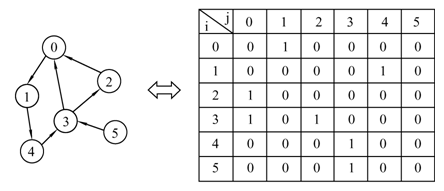
\includegraphics[width=3.71875in,height=1.60417in]{png-jpeg-pics/56BEF531A2AC657890949C5D11585A83.png}\\
}

{邻接矩阵的结构型定义如下:}{}{}{~}

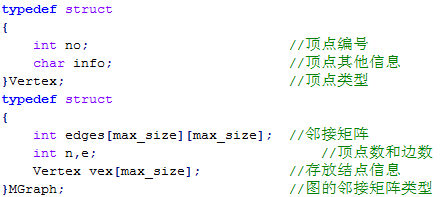
\includegraphics[width=3.70833in,height=1.63542in]{png-jpeg-pics/4FD252811BCF77D0A40599876B04AFB9.png}

{\textbf{2. 邻接表}}

{邻接表是图的链式存储结构。对每个顶点建立一个单链表,每个单链表的第一个结点存放顶点信息,其余结点存放边信息。如下图所示。}

{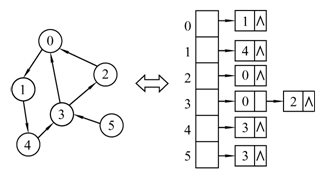
\includegraphics[width=3.70833in,height=2.06250in]{png-jpeg-pics/9403C7B366EB7BD65BE09160658072C6.png}\\
}{邻接表存储表示的定义如下:}

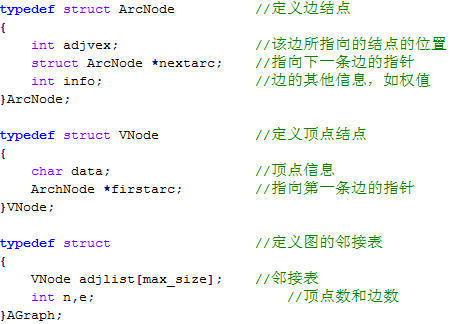
\includegraphics[width=3.70833in,height=2.65625in]{png-jpeg-pics/FBBDB091E668B536041132EA0D998D47.png}
